\documentclass[12pt]{article}
\usepackage[english]{babel}
% \usepackage[utf8x]{inputenc}
\usepackage[T1]{fontenc}
\usepackage{scribe}
\usepackage{listings}
\usepackage{fullpage}
\usepackage{amsfonts}
\usepackage{amssymb}
\usepackage{booktabs}
\usepackage{subcaption}
\usepackage{hyperref}
\hypersetup{
    colorlinks=true,
    linkcolor=blue,
    filecolor=magenta,      
    urlcolor=cyan,
    pdftitle={Overleaf Example},
    pdfpagemode=FullScreen,
    }
\usepackage{xurl}
\usepackage[svgnames]{xcolor}
\usepackage{color}
% \definecolor{light-gray}{gray}{0.90}
% \lstset{backgroundcolor=\color{light-gray},showlines=true}

% \usepackage{xcolor}
% \usepackage{listings}

% \lstdefinestyle{BashInputStyle}{
%   language=bash,
%   basicstyle=\small\sffamily,
%   numbers=left,
%   numberstyle=\tiny,
%   numbersep=3pt,
%   frame=tb,
%   columns=fullflexible,
%   backgroundcolor=\color{yellow!20},
%   linewidth=0.9\linewidth,
%   xleftmargin=0.1\linewidth
% }

\usepackage{minted}
\setminted{fontsize=\footnotesize, baselinestretch=1}

\Scribe{}
\Lecturer{Queenie Qiu, John Raiti. Student: \textbf{Shucheng Guo}}
\LectureNumber{7}
\LectureDate{DATE: March 2nd. 2023}
\LectureTitle{Pick and Place tasks and Arm Motion Planning}

\lstset{style=mystyle}

\begin{document}
	\MakeScribeTop


\section{Learning Objectives}

\begin{enumerate}
    \item Learn about waypoint generation in robotic arm trajectories and motion planning.
    \item Implement code to perform pick and place tasks in a recycle-sorting scenario.
\end{enumerate}


\section{Creating a robotic arm trajectory from waypoints}

\subsection{Trajectory planning with Bezier curve in Cartesian space for Kinova arm}

\textbf{Instruction:}
There are many trajectory planning strategies among which Bezier curve is one that is easy to apply and ideal for applications requiring a smooth trajectory. A Bezier curve is a mathematical curve defined by a series of control points, which determine the shape of the curve. The curve starts at the first control point and ends at the last control point, but it can bend and twist in any way that is defined by the other control points.

\begin{figure}[H]
    \centering
\includegraphics[width=12cm]{images/bezier.png}\vspace{-10pt}
    \caption{Cubic Bezier curve with four control points}\label{fig:curves}
\end{figure}

During this session, we will guide the Kinova arm to follow a trajectory based on a Bezier curve, moving it from the Home position to the Vertical position. First, we will acquaint ourselves with the lab materials, starting with an Excel file employed to generate a trajectory using Bezier curves. 

\href{https://uwnetid-my.sharepoint.com/:x:/g/personal/mecu_uw_edu/ETBpJ3Zvj1BNi2nTQRjYhxgBhsA50Y1KB6yDVAq8hl8sTQ?e=CROl1g}{This Excel file} calculates interpolate points along the Bezier curve based on 4 input control points, with two possible output versions containing 11 or 21 points.

\begin{figure}[H]
    \centering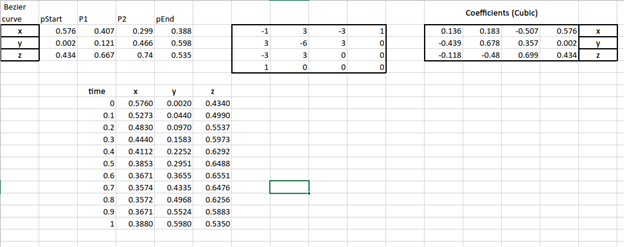
\includegraphics[width=10cm]{images/lab71.png}\vspace{-10pt}
    \caption{Bezier curve.}\label{fig:curves}
\end{figure}

Then spawn a robot in an empty world:

\begin{minted}{bash}
    $ roslaunch kortex_gazebo spawn_kortex_robot.launch arm:=
    gen3 gripper:=robotiq_2f_85
\end{minted}

We will use RViZ to select 4 points to generate a trajectory: Start, End, and 2 mid points. Use Home position as Start and Vertical as End. You need to find two intermediate poses (collect pose information from \mintinline{bash}{$ rosrun tf tf_echo base_link tool_frame}). 
The trajectories generated on the file are normalized in time ($0 \leqslant t \leqslant 1$). 

Select the version of your choice (11 or 21 points) and paste that information into you data.csv file. Once the data.csv file has been modified you can run the python script(plot\_trajectory.py) to plot the points in 3D for visualization.

\textbf{Tip}: you should replace (Ctrl + H) the tab spacing with a comma (,)

So far, we have handled the position of the end-effector’s pose along the trajectory with the Bezier curve. Next, we will need to generate
smooth changes between the orientations that differ at positions.

\begin{figure}[H]
    \centering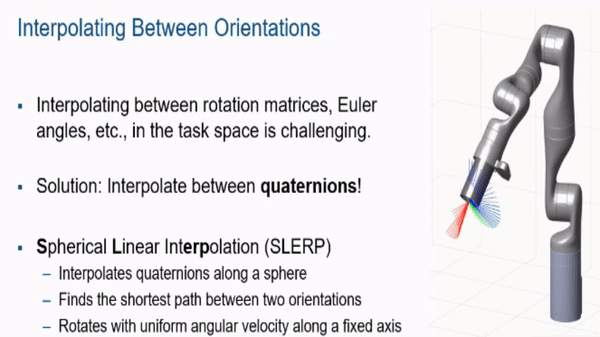
\includegraphics[width=8cm]{images/lab72.png}
    \caption{quaternions}\label{fig:curves}
    \end{figure}

For quaternion interpolation we will use one class of the python module pyquaternion. You can install it using pip:
\begin{minted}{bash}
    $ pip install pyquaternion
\end{minted}

The typical usage of pyquaternion that best suits our application is by declaring one quaternion for each start and end pose, and use one method that uniformly interpolates values in between:
\begin{minted}{python3}
    from pyquaternion import Quaternion
    qStart = Quaternion(w=<value>, x=<value>, y=<value>, z=<value>)
    qEnd = Quaternion(w=<value>, x=<value>, y=<value>, z=<value>)
    qList = Quaternion.intermediates(qStart, qEnd, <numIntermediates>, 
                include_endpoints=True)
\end{minted}

This chunk of the code is in trajectory\_from\_csv.py. This file combines the two composition of trajectory generation - positions along the path and quaternion interpolation. You can run the script and visualize the changes in both RViZ and Gazebo.

\textbf{Tip}: Execute the following command in your terminal to use pick\_and\_place.py class from terminal or import in different python files.
\begin{minted}{bash}
   $ export ROS_NAMESPACE="/my_gen3/"
\end{minted}

\textbf{Deliverables:}

\begin{enumerate}

    \item Submit the selected control points used to generate a (Bezier curve) trajectory to go from Home to Vertical position.
    
    \begin{table}[H]
        \centering
        \begin{tabular}{cccc}
            \toprule
            Points & \textit{x} & \textit{y} & \textit{z} \\ \midrule
            $P_0$ & 0.576 & 0.002 & 0.434 \\
            $P_1$ & 0.351 & 0.461 & 0.862 \\
            $P_2$ & -0.113 & 0.245 & 1.220 \\
            $P_3$ & -0.001 & -0.025 & 1.307 \\ \bottomrule
        \end{tabular}
        \caption{Control points in the Bezier curve trajectory}
    \end{table}
    
    \item Compare the path you created versus the path generated by Motion Planning in RViz starting from Home to Vertical. Please provide explanation when needed.
    
    \textbf{Answer: }The self-generated path has a smaller range of motion, while the one generated by MotionPlanning in RViz has a significantly bigger one.
    \\In calculating the way points, only the positions of the end effector are considered, so the trajectory of my own path is more smooth as expected. When planning with RViz, it seems that the joints are all moving at the same time, finding their shortest paths without prioritizing the end end effector.
    \\For the above reasons, path planning with different methods may lead to distinct performances. With Bezier curve, the end effector moves the shortest and most smooth path, while the joints maybe twisted and move a longer one. With RViz, wider space is required as the movement may be bigger, but from a holistic view, the whole execution is more smooth.
    
    \item Discuss the importance of complementing the trajectory generation process with the quaternion interpolation.
    
    \textbf{Answer: }As discussed above, generating a curved path doesn't guarantee smooth joint movement, and appropriate velocity change, which would cause trouble in path planning, like collisions and lack of accuracy. Applying quaternion interpolation, or SLERP in robotics is indispensable because it would find the shortest path between two orientations, and dictate the joints to rotate with uniform angular velocities along a fixed axis.
    
    \item Take a screenshot or save an image from your visualized trajectory from the plot\_trajectory script.
    
    \begin{figure}[H]
        \vspace{-10pt}
        \centering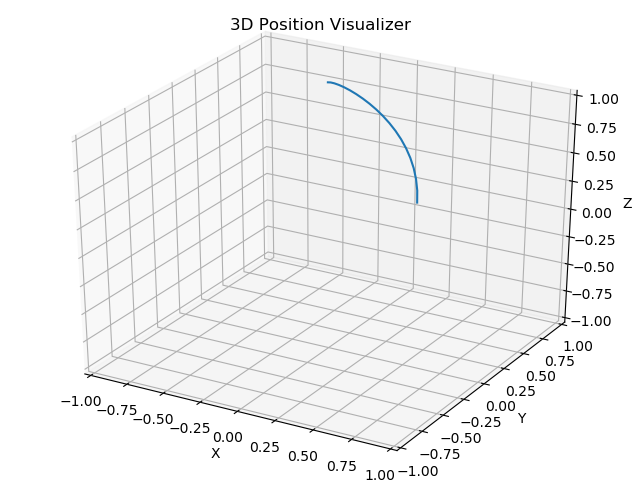
\includegraphics[width=12cm]{images/plot_traj.png}
        \caption{Visualizing the original trajectory plot}\label{fig:plot_traj}
    \end{figure}
    
    \item If you have any modifications to the script that would result in a better visualization experience, propose them here and take a second screenshot.
    
    \begin{figure}[H]
        \vspace{-10pt}
        \centering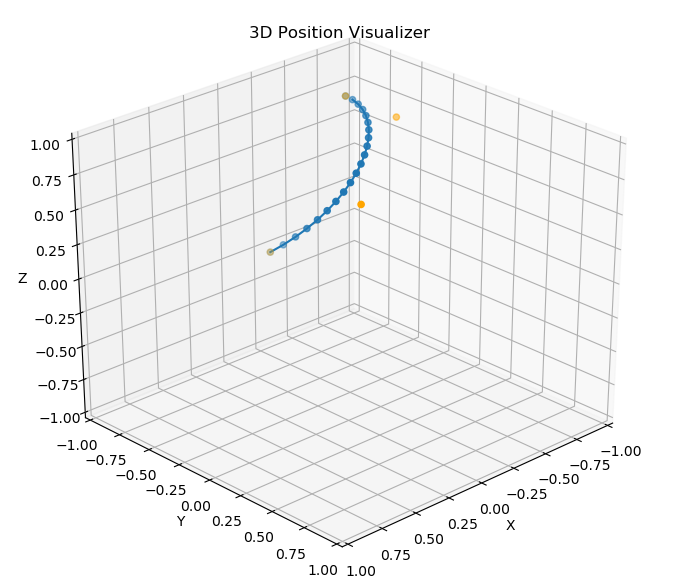
\includegraphics[width=14cm]{images/plot_traj_mod.png}
        \caption{Visualizing improved trajectory plot with points}\label{fig:plot_traj_mod}
    \end{figure}

    \textbf{Answer: }Compared to the original plot, where only the final trajectory is present, the enhanced plot comprises of four control points, 21 waypoints, and the line connected by the dots. The plot looks very much like the curve in \ref{fig:curves}, whose shape is determined by a series of control points.

\end{enumerate}
    
%     \item (Extra credit) Generate trajectory points with the quintil polynomial formula using the provided class:
    
%     Example usage of quintic polynomial class:
%     \begin{minted}{bash}
% >> from quintic_poly_class import quintic_polynomial
% >> lat_qp = quintic_polynomial(xStart, vStart, aStart, xEnd, vEnd, aEnd, Ti)
% >> for t in np.arange(0.0, Ti, deltaT)]
% >>	q = q.append(lat_qp.calc_point(t))
% >>	q_d = q_d.append(lat_qp.calc_first_derivative(t))
% \end{minted}
%     \end{enumerate}

\section{Pick and Place task with obstacle avoidance}

\textbf{Instructions:}
We have now become acquainted with all the aspects related to the arm's kinematics, trajectory planning, and the use of joint angles (configuration space) or end-effector poses (task space) to direct the robot's movements. In this section, we will apply all of these elements to a sorting task, which involves picking up cubes of different colors and placing them on top of the corresponding bins. It should be noted that the simulated environment includes walls that require careful planning to avoid collisions.

\begin{figure}[H]
    \vspace{-10pt}
    \centering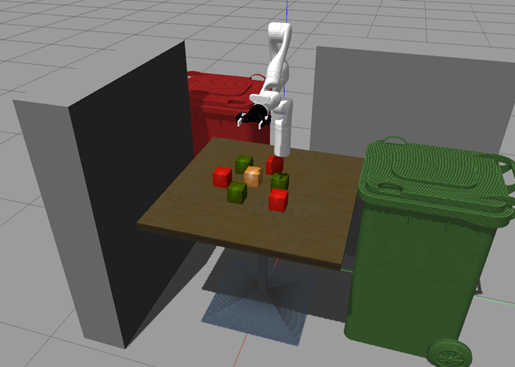
\includegraphics[width=12cm]{images/lab73.png}
    \caption{The planning scene}\label{fig:planning}
    \end{figure}


In the start\_gazebo.launch file (roscd kortex\_gazebo/launch) add the following argument to open the new generated world:

\begin{minted}{bash}
<arg name="world_name" value="<path to your Lab7_code folder>/sorting_world.sdf"/>
\end{minted}

Additionally, in the spawn\_kortex\_robot.launch file, modify the line that starts the RViZ node to include the configuration file provided in the lab materials:

\begin{minted}{bash}
<node name="rviz" pkg="rviz" type="rviz" args="-d 
<path to your Lab7_code folder>/pickandplace.rviz" if="$(arg start_rviz)"/>
\end{minted}

Once you have completed those changes, run the following command:

\begin{minted}{bash}
$ export GAZEBO_MODEL_PATH=$GAZEBO_MODEL_PATH:<path to your Lab7_code folder>
$ roslaunch kortex_gazebo spawn_kortex_robot.launch arm:=gen3 gripper:
=robotiq_2f_85 z0:=0.775
\end{minted}

Drawing on your prior knowledge of trajectory planning from the previous section, as well as your experience from the previous lab assignment, think about how the sorting task can be broken down into smaller sub-tasks, such as sorting the green cube and sorting the red cube. Additionally, the process for sorting the green cube can involve the same steps as the pick-and-place task from lab 6. To refresh your memory, the pick-and-place task involves the following steps:

\begin{enumerate}
    \item Reach position above the center of the object to be picked with gripper oriented
    \item Adjust gripper to open or semi-open state.
    \item Decrease the end-effector’s z-value position
    \item Close gripper to grasp object.
    \item Reach position above the desired location to place the object with gripper oriented.
    \item Decrease the end-effector’s z-value position
    \item Open gripper to release object.
    \item Increase the end-effector’s z-value position to clear the object
    \item Return to home position.
    
\end{enumerate}

However, for sorting the cubes, you should consider finding waypoints that won't hit the walls, and generating trajectories that guarantee a successful movement between picking and placing.


We have only started covering the many functionalities of MoveIt! You can use the following \hyperlink{http://docs.ros.org/en/melodic/api/moveit_tutorials/html/doc/quickstart_in_rviz/quickstart_in_rviz_tutorial.html}{link} to go through their documentation.
There are very valuable resources in \hyperlink{https://www.mathworks.com/videos/trajectory-planning-for-robot-manipulators-1556705635398.html}{Mathworks}. Those resources are part of a commercial product, but it is worth looking into them.
If you require additional information about the pyquaternion module, visit their \hyperlink{http://kieranwynn.github.io/pyquaternion/}{documentation}.\\

\textbf{Deliverables:}

\begin{enumerate}

    \item Provide a walkthrough of your process to complete the sorting task:
    
    \begin{enumerate}

        \item What sub-tasks did you select to divide the sorting task into? What did each sub-task entail?	Discuss the steps within each of your sub-tasks
        
        \begin{enumerate}
            \item Approach the object to pick
            \begin{itemize}
                \item Reach position above the center of the object to pick
                \item Adjust the gripper to open or semi-open state
                \item Lower the end effector by decreasing \textit{z} to approach object
            \end{itemize}
            \item Pick the object
            \begin{itemize}
                \item Adjust the gripper to close state
                \item Raise the end effector by increasing \textit{z} to move object up
            \end{itemize}
            \item Move it to the goal position
            \begin{itemize}
                \item Calculate waypoints based on current and goal pose
                \item Plan trajectories with waypoints to avoid crashes
                \item Execute the movement and reach position above the desired location
            \end{itemize}
            \item Place the object
            \begin{itemize}
                \item Lower the end effector by decreasing \textit{z} to place object
                \item Adjust the gripper to open state
                \item Raise the end effector by increasing \textit{z} to clear object
            \end{itemize}
            \item Return to home position
        \end{enumerate}
        
        \item Mention some of the challenges and how you addressed them.
        
        \textbf{Answer: }One of the biggest challenges I faced was not being able to initialize RViz. After running the commands in the terminal to instantiate the arm in Kortex\_Gazebo, an error would pop up, saying the parameters aren't found. This issue persisted over a week and was resolved by reinstalling the operating system and modifying the xacro parts in the launch files.
        \\Another difficulty was to plan a route without the risk of crashing and execute with python. It was achieved by calculating waypoints with self-selected control points in the Belzier curve. Firstly, I determined the current and goal positions, the states after picking and before placing the object; then I moved the arm to up above where it wouldn't hit the walls and recorded two points as the midway control points. Waypoints were then calculated based on the four control points and the trajectories were executed without errors.
        
    \end{enumerate}

    \item Report values of interest used to complete the task:
    
    \begin{enumerate}

        \item Poses of the cubes, the bins, the selected waypoints, and desired placing location.
        
        \textbf{Answer: }Below is an instance of a part of the sorting task, where the furthest red cute is picked from the table and placed on the reb bin. Other points of interest outside of this task aren't included to prevent confusion.
        
        \begin{table}[H]
            \caption{Pose information of locations of interest}
            \begin{subtable}{.32\linewidth}
                \centering
                \caption{Red cube}
                \begin{tabular}{ccc}
                    \toprule
                    \textit{x} & \textit{y} & \textit{z} \\\midrule
                    0.526 & 0.126 & 0.774 \\\bottomrule
                \end{tabular}
            \end{subtable}
            \hfill
            \begin{subtable}{.32\linewidth}
                \centering
                \caption{Red bin}
                \begin{tabular}{ccc}
                    \toprule
                    \textit{x} & \textit{y} & \textit{z} \\\midrule
                    -0.798 & -0.837 & 0.015 \\\bottomrule
                \end{tabular}
            \end{subtable}
            \hfill
            \begin{subtable}{.32\linewidth}
                \centering
                \caption{Destination}
                \begin{tabular}{ccc}
                    \toprule
                    \textit{x} & \textit{y} & \textit{z} \\\midrule
                    -0.432 & -0.429 & 0.992 \\\bottomrule
                \end{tabular}
            \end{subtable}
        \end{table}

        \begin{figure}[H]
            \vspace{-10pt}
            \centering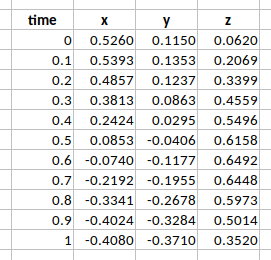
\includegraphics[width=5cm]{images/waypoints.png}
            \caption{Waypoints between approaching and placing object locations}\label{fig:waypoints}
        \end{figure}

        \item Selected height to approach object and place locations.
        
        \begin{table}[H]
            \caption{Pose height}
            \centering
            \begin{tabular}{ccc}
                \toprule
                \textbf{State} & \textit{Approach} & \textit{Place} \\\midrule
                \textbf{Height} & 0.062 & 0.280 \\\bottomrule
            \end{tabular}
        \end{table}

        \item Percentage of the gripper’s open/close position.
        
        \begin{table}[H]
            \caption{Gripper position}
            \centering
            \begin{tabular}{ccc}
                \toprule
                \textbf{State} & \textit{Open} & \textit{Close} \\\midrule
                \textbf{Percentage} & 0 & 30\% \\\bottomrule
            \end{tabular}
        \end{table}
        
    \end{enumerate}
    
    \item Record a video of the entire sorting task or select a specific portion of the task of the robot carrying out the necessary movements. You can choose to control the Kinova arms using Rviz or by writing code. If you opt for the latter, you can refer to the "pick\_and\_place.py" file for guidance.
    
    \href{https://drive.google.com/file/d/1WHiMvIzTKDBX92PTeloq5f1X7C0vTkVE/view?usp=share_link}
    {Google Drive link to the video of sorting a red cube}

\end{enumerate}

\end{document}